\chapter{Introduction}
First we give a primer on domain adaptation and then an introduction to optimal transport theory.

\section{Motivation}

In statistical learning theory, many results study the problem of estimating when a hypothesis from a select hypothesis class produces a low true risk. This is often expressed as a generalization bound on the true risk. The typical generalization problem assumes that the training and test distributions are identical. 

One example of this is facial recognition, where an image classification model is learned on a community and is then used to classify those in another community who may have different facial features. The image recognition performance will deteriorate when the classification model does not account for the disparity between training and test distributions \cite{Redko2017}.

Another instance in which this assumption is violated is the spam filtering problem. A given user will be targeted with spam messages depending on his browsing history. If a working professional sets up his corporate mailbox on his home computer and transfers his settings, many personal emails he may want could be perceived as spam by an algorithm that learned preferences from professional communications. A classifier distinguishing spam from non-spam may not perform as well on another user if it does not adapt to different circumstances \cite{Redko2017}.

\begin{figure}
	\centering
	
\includegraphics[width=0.7\linewidth]{pictures/anti-spam-filtering-techniques.png}
	\caption{One application of transfer learning: spam filtering.}
	\label{fig:datree}
\end{figure}

Such examples motivate the domain adaptation problem and extend traditional learning paradigms. For the rest of this dissertation, we investigate the scenario where a model may be learned on one distribution but evaluated on another.

\section{Background}
For the applications considered above, the goal is to find a model that remains robust under changes in the environment. In other words, if a model is learned from the source, we want to measure how well it performs on the target domain. Formally, we describe this as follows

\begin{theorem}[Transfer learning]
	Let $S$ be a source data distribution called the source domain and $T$ be a target data distribution called the target domain. Consider $X_S\times Y_S$ as the source input and output spaces and $X_T\times Y_T$ as target input and output spaces. Denote $S_X$ and $T_X$ to be the marginal distributions of $X_S$ and $X_T$ and by $t_S$ and $t_T$ the source and target learning tasks depending on $Y_S$ and $Y_T$ respectively. We seek to improve the performance of $f_{T}:X_T\to Y_T$ for $t_T$ using information gained from $S$ where $S\neq T$.
\end{theorem}

\subsection{Transfer learning scenarios}
 
Furthermore, we have the following types of learning:
\begin{itemize}
	\item Inductive transfer learning. $X_S=X_T$ but $t_S\neq t_T$.
	\item Transductive transfer learning. $X_S\neq X_T$ but $t_S=t_T$.
	\item Unsupervised transfer learning. $t_S\neq t_T$ and $X_S\neq X_T$.
\end{itemize}

The category we focus on is transductive transfer learning, which we hereafter call domain adaptation.

% TODO: \usepackage{graphicx} required
\begin{figure}
	\centering
	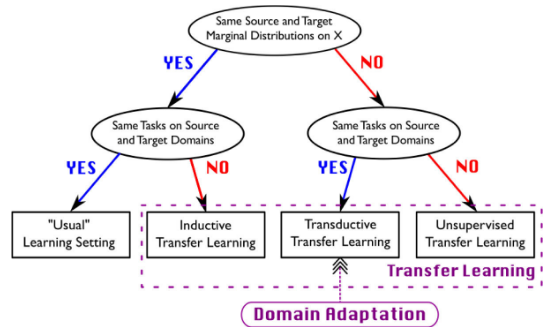
\includegraphics[width=0.7\linewidth]{pictures/DA_tree}
	\caption{Positioning of Domain Adaptation compared to other learning techniques (Redko).}
	\label{fig:datree}
\end{figure}

From a probabilistic point of view, we can categorize our problem via the causal link between labels and instances.

\begin{itemize}
	\item $X\to Y$ problems where the class label is causally determined by instance values. This labeling comes up in image classification where the object description determines the label. The joint distribution can be decomposed into $P(X,Y)=P(X)P(Y|X)$.
	\item $Y\to X$ where this is the reverse. Class labels causally determine instance values. A good example here is in medical applications where we observe disease symptoms but want to predict the disease \cite{Redko2017}. The joint decomposition here is $P(X,Y)=P(Y)P(X|Y)$.
\end{itemize}

It follows that we can categorize different types of transfer learning scenarios based on the probabilistic point of view. The following are some such scenarios:

\begin{itemize}
	\item Covariate-shift
	$P(X_S)\neq P(X_T)$ but $P(Y_T|X_T)= P(Y_S|X_S)$
	
	This is a case of the $X\to Y$ problem where $X_S\not\equiv X_T$ while $Y_S|X_S \equiv Y_T|X_T$. Here, the marginal distributions between the source and target are different while the predictive behavior stays the same. One example of this is the Office/Caltech dataset \cite{Caltech} with domains:
	
	\begin{enumerate}
		\item Amazon images from online merchants.
		\item Low-quality webcam images.
		\item High-quality images taken with a DSLR.
		\item Images from Caltech dataset for object recognition.
	\end{enumerate}
	
	% TODO: \usepackage{graphicx} required
	\begin{figure}
		\centering
		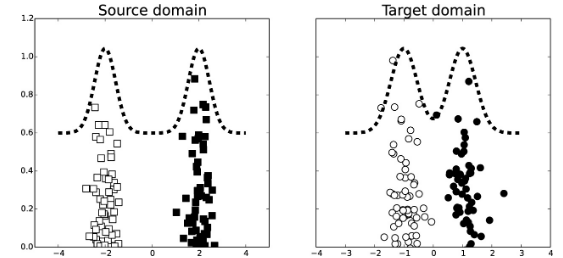
\includegraphics[width=0.7\linewidth]{pictures/covariate_shift}
		\caption[Covariate shift illustration.]{Covariate shift}
		\label{fig:covariateshift}
	\end{figure}

	Solving the covariate shift problem involves a reweighting as seen by the following:
	
	\begin{align*}
	R^l_T(h) &= \E_{(x,y)\sim T} l(h(x),y) \\
	&= \E_{(x,y)\sim T} \frac{S(x,y)}{S(x,y)}l(h(x),y) \\
	&= \E_{(x,y)\in X\times Y} T(x,y)\frac{S(x,y)}{S(x,y)}l(h(x),y) \\
	&= \E_{(x,y)\sim S} \frac{T(x,y)}{S(x,y)}l(h(x),y) \\
	&= \E_{(x,y)\sim S} \frac{P(X_T)}{P(X_S)}l(h(x),y)
	\end{align*}
	
	where the last equality uses the fact that $P(Y_T|X_T)=P(Y_S|X_S)$.
	
	
	\item Target-shift
	$P(X_T|Y_T)\neq P(X_S|Y_S)$
	
	These occur in $Y\to X$ problems. In this case, $Y_S\not\equiv Y_T$--the target distributions are different. Generally, this occurs when different sampling methods are used for the source and target datasets.
	
	\begin{figure}
		\centering
		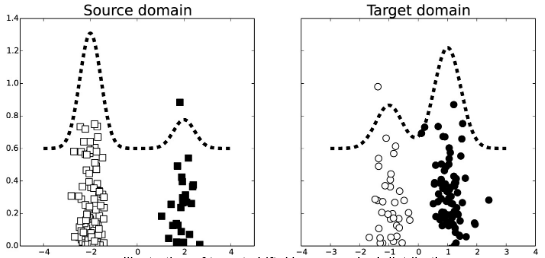
\includegraphics[width=0.7\linewidth]{pictures/target_shift}
		\caption[Target shift illustration.]{Target shift}
		\label{fig:targetshift}
	\end{figure}
	
	\item Concept shift
	$P(X_T,Y_T)\neq P(X_S,Y_S)$ This occurs both in $X\to Y$ and $Y\to X$ problems when $P(Y_S|X_S)\neq P(Y_T|X_T)$ and $P(X_S|Y_S)\neq P(X_T|Y_T)$ respectively.
	\item Sample-selection bias
	
	Here, the source and target distributions differ because of a latent variable that excludes some sample observations conditional on their labeling or nature. For example, if we are classifying images of people, we may discard images that are unclear. This exclusion leads to a sample-selection bias, since some devices may take less clear pictures by default.
	
	\item Ideal joint error.
	We may claim the existence of a low-error hypothesis for both the source and target domain. Usually, this is characterized by
	\[
	\lambda_{\mathcal{H}}=\min_{h\in \mathcal{H}} R_S(h)+R_T(h)
	\]
	
\end{itemize}

As a side-note, there are three predominant algorithmic techniques used for domain adaptation. They are

\begin{enumerate}
	\item Reweighting the source labeled examples to be more similar to the target examples. This is done in cases such as covariate shift.
	\item Iteratively ``auto-labeling" target examples. Here, a model is learned from labeled examples and then automatically labels some target examples. We then learn a new model from the new labeled examples.
	\item Finding a common representation space. In this situation, we find a space where the source and target domains are close while maintaining a good performance on the source domain task.
\end{enumerate}

\subsection{Divergence between domains}

In domain adaptation, we must define a dissimilarity measure between source and target domains. Unlike classical supervised learning, transfer learning involves a discrepancy between the two domains. There are many metrics, such as Hellinger distance total-variation distance, Renyi divergence, or Wasserstein metric, that exist to measure such a discrepancy, and the choice of metric can impact the behavior of the labeling function. \cite{Redko2017}

Often, one wants to prove that a divergence measure can relate errors between source and target domains. This relation means we can establish error guarantees by minimizing the divergence between the source and target distributions.

Along with analyzing existing divergence measures, one may also design a new divergence measure suitable for domain adaptation. This is done when a divergence measure is too difficult to compute empirically.  Additionally, we investigates a new specific divergence measure in Chapter 3.

In the subsequent paragraphs, we discuss seminal work in this area of research. We do this to better demonstrate what we mean by relating errors between domains with respect to a divergence measure.

\subsection*{A First Theoretical Analysis}
From a theory perspective, the seminal work was done by Ben-David et al. In their work, they considered a binary loss function in a binary classification by setting and proposing the $L^1$-distance \cite{Ben-David2007}.

First, we provide some definitions.

\begin{definition}{Rademacher complexity}
	
	Given a sample $S=(z_1, z_2, \dots, z_m) \in Z^m$, and a class $F$ of real-valued functions defined on a domain space $Z$,
	\[
	\operatorname{Rad}_S(F) 
	= 
	\frac{1}{m}
	\operatorname{E} \left[
	\sup_{f \in F}
	\sum_{i=1}^m \sigma_i f(z_i) 
	\right]
	\]
\end{definition}

\begin{definition}{Shattering}
	
	A family $H$ shatters a set $S \subseteq \mathcal{X}$ if for every subset $T \subseteq S$ there exists a function $h \in H$ such that $h(s) = 1_{s \in T}$ for all $s \in S$, that is, $h(s) = 1$ if $s \in T$ and $h(s) = 0$ if $s \in S \setminus T$.
	
	Intuitively, we say that $H$ shatters some set $S \subseteq \mathcal{X}$ if we can realize any labelings on $S$ using functions from $H$.
	
\end{definition}

\begin{definition}{VC Dimension}
	 
	 The VC dimension of a set of hypothesis functions $H$ is the cardinality of the largest set which $H$ can shatter.
	
\end{definition}

\begin{definition}{$\mathcal{H}$-divergence}
	
	Denote $\mathcal{A}$ the set of measurable subsets under two probability distributions $\mathcal{D}$ and $\mathcal{D'}$. Then the $\mathcal{H}$-divergence is defined as
	\[
	d_{1}(\mathcal{D},\mathcal{D'}) = 2 \sup_{A\in \mathcal{A}} \left| P_D(A)-P_{D'}(A) \right| .
	\]
\end{definition}

This one compares how two classifiers disagree on both domains. Here, it finds the pair of classifiers with the largest disparity in disagreements between the source and target domains.

Using this notion of distance, Ben-David et al. derived the first generalization bounds.

\begin{theorem}{Generalization bound with respect to $\mathcal{H}$-divergence \cite{Ben-David2007}}
	
	Let $l$ represent the $0-1$ loss function and $f_S,\,f_T$ the source and target true labeling functions respectively.
	\[
	R_T^{l}(h) \leq R_S^{l}(h) + d_1(X_S,X_T) + \min \left\{ \E_{x\sim X_S} [\left\|f_S(x)-f_T(x)\right\|], \E_{x\sim X_T} [\left\|f_S(x)-f_T(x)\right\|] \right\}
	\]

\end{theorem}

This was the first theoretical generalization bound, and it had some flaws. In practice, one may want to obtain finite-sample estimates, but that isn't possible with $\mathcal{H}$-divergence. Also, the $\mathcal{H}$-divergence does not incorporate the hypothesis class. Both of these issues are resolved with the introduction of another type of divergence: the symmetric difference hypothesis divergence.

\begin{definition}{Symmetric difference hypothesis divergence}
	\[
	D_{\mathcal{H}\Delta \mathcal{H}}(S,T) = 
	2 \sup_{h,h'\in \mathcal{H}} \left| P_S[h(x)\neq h'(x)] - P_T[h(x)\neq h'(x)] \right| 
	\]
\end{definition}

\begin{theorem}
	Here, $\hat{S},\hat{T}$ are independent size-$m$ samples drawn from $S$ and $T$ respectively. For $\delta\in (0,1)$, the following holds with probability at least $1-\delta$:
	
	\[
	D_{\mathcal{H}\Delta \mathcal{H}}(S,T) \leq \hat{D}_{\mathcal{H}\Delta \mathcal{H}}(\hat{S},\hat{T}) + 
	4 \sqrt{\frac{2 VC(\mathcal{H}) \log(2m) + \log(2/\delta)}{m}}
	\]
\end{theorem}

The above tells us that, for a finite $VC$ dimension class $\mathcal{H}$, the empirical $\mathcal{H}\Delta \mathcal{H}$ divergence is a good estimate for its true variant.

Furthermore, one can compute the empirical divergence. Ben-David then obtained a bound for risk on the target domain that involved the empirical divergence.

\begin{theorem}
	Let $\lambda^* = \min_{h\in \mathcal{H}} R_S(h)+R_T(h)$ be the minimum joint risk.
	With probability at least $1-\delta$:
	
	\[
	R_T^l(h) \leq \hat{R}_S^l(h) + \frac{1}{2}D_{\mathcal{H}\Delta \mathcal{H}}(\hat{S},\hat{T}) + \lambda^{*} + 
	O \left( \sqrt{\frac{VC(\mathcal{H}) \log(m) + \log(2/\delta)}{m}}\right) 
	\]
\end{theorem}

One sees here that the bound relies on a notion of divergence between the two domains, as stated earlier, along with a divergence between the hypothesis and true labeling function.

Of note here is that the risk bound presented is only relevant if the optimal joint risk is controlled.

\subsection*{Critique of $\mathcal{H}\Delta\mathcal{H}$-divergence}

A flaw of the $\mathcal{H}\Delta\mathcal{H}$-divergence is that it relies on a specific loss function (0-1 loss). Contrarily, one may want to work with a more general loss function. This desire motivated other work by Mohri and Mansour to use Renyi and $\mathcal{Y}$-discrepancy distances.

\begin{definition}{Renyi divergence}
	\[
	D_{\alpha}(p,q) = \frac{1}{\alpha-1} \log_2 \int_{\mathcal{X}} p^{\alpha}(x)/q^{\alpha-1}(x) \, dx,
	\]
	where $\alpha$ denotes its order. When $\alpha=1$, the Renyi divergence is equivalent to the Kullback-Leibler divergence.
\end{definition}

\begin{definition}{$\mathcal{Y}$-Discrepancy}

	Let $f_P$ and $f_Q$ be the labeling functions on $P$ and $Q$. Then the $\mathcal{Y}$-discrepancy between domains $(P,f_P)$ and $(Q,f_Q)$ is
	\[
	\textrm{disc}_{\mathcal{Y}}(P,Q) = \sup_{h\in H} \abs{\mathcal{L}_Q(h,f_Q)-\mathcal{L}_P(h,f_P)}
	\]
\end{definition}

In the majority of this dissertation, we study divergences inspired by optimal transport theory. This brings us to the next section, which introduces some of the foundational material on Wasserstein spaces.

\section{Brief Introduction to Optimal Transport}

\subsection*{Monge Problem}

In 1781, Gaspard Monge asked how one can transport a pile of sand into a pit when both have equal volumes.

Intuitively, the goal is to minimize the expected ``cost" of moving the sand, and it turns out this has a mathematical formulation as follows:

Let $X$ be the space of sand, $Y$ be the space for the pit, and define a cost function $c:X\times Y\to \mathbb{R}$ that demonstrates the cost of moving a unit of sand $x\in X$ to a pit location $y\in Y$.

The choice of where to place a unit of sand can be represented as the function $T:X\to Y$, which has a total transport cost of
\[
\int_{X} c(x,T(x))\,d\mu(x).
\]

Here, the sand distribution and shape of the pit are represented by distributions $\mu$ and $\nu$, respectively.

Moreover, one cannot change the size of a sand particle, so the sand cannot be concentrated at a single point in the pit. In other words, the function $T$ must satisfy a mass-preservation requirement: the volume $\nu(B)$ of any region in the pit $B\subseteq Y$ must be the same as the volume of the sand moved into $B$.

Formally, we can write this as
\[ 
\mu(T^{-1}(B))=\nu(B) \text{ for all } B\subseteq Y
\] which we denote $T\#\mu=\nu$. We can also recognize this as $\nu$ is the push-forward measure of $\mu$ under $T$.

If $c$ and $T$ are measurable, and $\mu(T^{-1}(B))=\nu(B)$ for all measurable subsets $B$ of $Y$, then $T$ is a transport map. Normalizing $\mu$ and $\nu$ to be probability measures, the Monge problem finds the optimal transport map minimizing transport costs \cite{Panaretos2020}. 

\begin{definition}{Monge Problem}
	
	Let $T:X\to Y$ be a transport map with an associated total cost \[
	C(T) = \int_{X} c(x,T(x)) \,d\mu(x).
	\] where $\mu$ and $\nu$ are again the probability measures assigned to $X$ and $Y$.
	
	The Monge problem finds
	\[
	\inf_{T:T\#\mu=\nu} C(T).
	\]
\end{definition}

The Monge problem is very hard because the set of transport maps $\{T:T\#\mu = \nu\}$ is intractable to work with. Currently, if $\mu=\delta\{x_0\}$ is a Dirac measure and $\nu$ is not, then no transport maps exist.

But what if we can split the mass of sand particles? That is to say, what if we don't have the strict conditions as above. This brings us to the Kantorovich relaxation.

\subsection*{Kantorovich Relaxation}
For each point $x\in X$, a probability measure $\mu_x$ defines how the mass at $x$ is split. If $\mu_x = \delta\{y\}$ for $y\in Y$, then all the mass at $x$ is sent to $y$.

Represent $\pi$ to be the joint probability measure on $X\times Y$, where $\pi(A\times B)$ is the amount of sand moved from $A\subseteq X$ to $B\subseteq Y$. The total mass sent from $A$ is $\pi(A\times Y)$ and the total moved into $B$ is $\pi(X\times B)$. Such a measure $\pi$ is called a  transference plan when
\begin{align*}
\pi(A\times Y) = \mu(A),\quad A\subseteq X \\
\pi(X\times B) = \nu(B),\quad B\subseteq Y
\end{align*}

where $A$ and $B$ are Borel sets. The set of transference plans is denoted $\Pi(\mu,\nu)$.

\begin{definition}{Kantorovich Problem}
	
	Let $\pi\in \Pi(\mu,\nu)$ be a transference plan with an associated total cost \[
	C(\pi) = \int_{X\times Y} c(x,y) \,d\pi(x,y).
	\]
	
	The Kantorovich problem solves for the optimal plan given by
	\[
	\inf_{\pi\in \Pi(\mu,\nu)} C(\pi).
	\]
\end{definition}

\subsection*{Probabilistic Interpretations of Monge and Kantorovich Problems}
We can view the above optimization problems from a probabilistic perspective. The Monge solution minimizes  $\E_{X}[c(X,T(X))]$ over $T$ (measurable) whereas the Kantorovich solution minimizes $\displaystyle\E_{\pi\in \Pi(\mu,\nu)}[c(X,Y)].$ We call $\pi \in \Pi(\mu,\nu)$ a coupling between $X$ and $Y$.

\subsection*{A Divergence Measure Inspired by Optimal Transport}
If $X=Y$, then we can define a distance between measures $\mu$ and $\nu$ using a special cost function $c$. 

Let $c(x_1,x_2) = [d(x_1,x_2)]^p$, where $d(x_1,x_2)$ denotes the distance between $x_1$ and $x_2$ and $p$ is a real-valued constant

\begin{definition}{Wasserstein Distance of Order p}
	\[
	W_p(\mu,\nu) = \left( \inf_{\pi\in \Pi(\mu,\nu)} \int_{X\times X} d(x_1,x_2)^p \,d\pi(x_1,x_2)\right)^{1/p} = \left( \inf_{\pi\in \Pi(\mu,\nu)} \E_{\pi}[d(x_1,x_2)^p] \right)^{1/p} .
	\]
\end{definition}

With this being said, let's begin.